\section{Harmonics}

In order to win the daily battle\footnote{\url{https://gornahoor.net/?p=3005}}, we may resort to any number of tactics which can strengthen the ``core" of man by magnetizing the higher centers of his personality, including plain music\footnote{\url{http://www.youtube.com/watch?v=IoSuyUFiEYo}}. As several correspondents on this site have suggested, there may be a harmonic basis for this in Solfeggio notes\footnote{\url{http://www.youtube.com/watch?v=9su8OVjewS0&feature=related}}. Counterpoint, basso profundo, \& harmonics may provide us with a means of understanding the polyphony (and seeming polytheism) of Life. Music teaches us to eschew the demon of dialectics, as well as helping to cure the demon of the noonday sun\footnote{\url{http://www.johnsanidopoulos.com/2012/01/their-noonday-demons-and-ours.html}}. We can use it to see harmony, rather than conflict, or conflict-in-harmony.

The ``diamond self" (it is averred) is the opposite path from the dissolution of the self and resolution of the new Self in Christ; even Tomberg emphasizes this in his \emph{Meditations}, that the path of the East is to withdraw into the self, and it is valid, but not highest. After all, there are many stars in the night sky, all of them real, no doubt many glorious, but there is but one North Star which we may steer by in our humanity. And this, in fact, is true. The Medieval Era, whatever else it is, is the paramount Age of Man, Man as Man. Just as ancient times were the times of the gods, and modern times are the times of the robot and the beast, the Middle Ages were the time of Man.  Likewise, Christianity is (or should be) the religion best calculated to preserve that which makes us human, as a trophy and shield to bear into heaven.

\begin{wrapfigure}{rt}{.3\textwidth}
 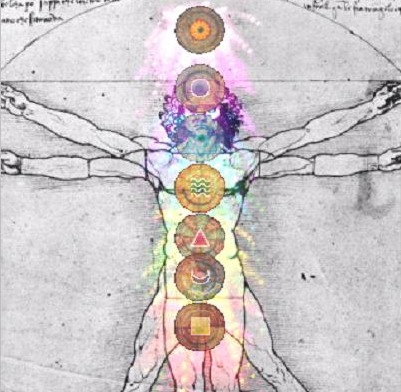
\includegraphics[scale=.5]{a20120107Harmonics-img001.jpg} 
\end{wrapfigure}

However, what if ultimately (in the post-mortem states) these two paths, the path of the Diamond, and the path of the Hermit, are not (in fact, finally) separated? We already intuit this to be so, since Christianity claims that Christ's final act will be the conquest of Death and Hell, the Recapitulation of all things within the Logos, where, at the end of Time, he will surrender his \emph{imperium} back to the Father (see Colossians). Will the Logos, through whom all things were created, lose something given to His care? Thus, the survival of one avatar of Man upon the path of the Hermit means that those of the Diamond Self, the wandering stars, will be at the end of time, gathered back into the fold. It is possible to be a Super-Man, your own Christ, because of the final Christ, found not during your stay in the vale-of-soul-making\footnote{\url{http://academic.brooklyn.cuny.edu/english/melani/cs6/keatsltr.html}}, but later, in the houses-of-many-mansions, at the end of time.

We see this to be so from the breath. Man breathes in, then exhales. With close attention, one can tell that it is the ``breathing out" (or surrender) which collapses the chest and pulls the life down into the spiritual heart, whereas the breathing in raises the spirit in exaltation. But then again, in effect, the breathing in is also (in its way) a prayer to above, although it is more aggressive in taking. Likewise, one can see that breathing out might be taken as a rejection of God, or a letting go of even Him. The breath, although in two paths, is finally One. There is one breather, one breath.

The path of the diamond self is simply the continuation of existence (or a certain form of it) in the post-mortem state, indefinitely, which will trace its own way back to God. The path of hermit is actually swifter, though it seems to tarry in the fields and byways and inns of the ring of the world. One ``makes haste, slowly".

Which is better? Which is more noble? Since they are finally the same, the choice is left up to us: ``Whatever you bind on earth, will be bound in heaven; whatever you loose on earth, loosed in heaven…be careful how you judge – which ever way a man judges, in that way shall he also be judged…" Does the Super-man wish to be without the Self of higher Selves? How can he be God, if there is no God? What else does it mean, to say, the Lord has given him a name above every names, highly exalted? There are many little Christs; if there were not, how could we picture the Exalted One?

The chakras correspond to the sacred Solfeggio notes (the glands of the endocrine system are externalizations of the inner pathways, coagulations of serpentine energy which imitates the sacred network), and this forms the Kundalini energy trail. Here is Evola:

\begin{quotex}
Lightning moves downwards, which Evola explains it is a sort of ``command of those who have reached this supreme plane is like a thunderbolt that travels along the entire hierarchy, starting from the top until it reaches the vibrations at the very bottom, which shape matter. This is the so-called vajra-vak, the diamond-thunderbolt of the living word." (TYoP, page 13) The cyclical nature then allows the initiate to `shape matter'. Then he begins again at the bottom, as Evola describes the process of upward moving chakras: ``Through the earth chakra one acquires an extraordinary material strength. Through the water chakra one may acquire youthful energies, thus neutralizing the processes of aging and of organic decay (``The Water of Life"). Through the fire chakra one acquires the power of transforming and of dissolving the elements (this corresponds to the Hermetic saying \textit{solve et coagula})." (TyoP, page 184)

\flright{Source: \url{http://www.joanlansberry.com/wr-hekau/serp2of2.pdf}}

\end{quotex}
Those who wish to return from the pharoah's tomb bearing a forked stick with a brazier of fire on their head will have to ``wake up", which is to initiate their chakras. But how? Do we do this alone, or with others? With the Other? As a diamond-thunderbolt who utters the \emph{vajra-vak}, or as someone supplicating ``the Lord"?

Here is Tomberg's description\footnote{\url{http://www.eleggua.com/Objects/Tomberg-Spiritual_Basis.html}} of what happens in the Christian path, which many regard as ``Semitic":

\begin{quotationx}
The power which makes man into an upright, vertically oriented being entered into men following the Fall. In essence it was what today we usually call ``pride". The Bible shows the nature of this power by the words of the Tempter : ``Ye shall be as Gods." When pride entered into human nature through the Luciferic impulse, a vertical scream, from below upwards, came into being in the human organization. The physically perceptible expression of this scream is the backbone. What has formed itself physically into backbone consists astrally of \emph{pretensions of pride.} These pretensions have themselves as object : they feed on themselves. So arises the upward streaming swirling movement of the passion of pride. The form of the vertebral column is its physical expression.

Now the basic pre-condition for the Manas revelation is that a stream must come into being which goes in the opposite direction : from above downward. Regarded \emph{spiritually ,} it is the stream of revelation ; as soul-phenomenon, however, it is borne on the stream of \emph{humility.} But opposing it is the pride which lives in all human nature since the Fall.

Therefore, in order to make it possible, a purification of human nature must precede the Manas revelation. This purification consists in the dying out of pride in that part of the astral body required for cognition. Man has to submit to a process of \emph{humiliation} which brings the Manas organization to maturity. This humbling is accomplished as follows : The man who out of the forces of his consciousness soul has chosen the spirit will be, as it were, `incarcerated'. On the one hand, a protective wall will be erected around him against evil influences ; on the other hand, a dome arches over his head consisting of the \emph{silence of the spiritual world.} Thus arises an \emph{empty} space where the man is quite alone. This space is so empty that even evil cannot enter there. The man has an opportunity fully to experience his powerlessness and poverty. He also grows fully conscious of the nature of his personal feeling of pride in all its vanity, and the powerlessness of his pretensions. In this emptiness of soul and silence of the spirit, his pride gradually dies away — until one day the decisive hour arrives in which the man feels himself to be a broken hollow reed and finds no more strength in himself to stand upright in the world. For what has held him upright since time immemorial, the power of his pride, is now broken ; the core of life for his personality is wiped out. Then man experiences himself as \emph{so} empty that there remains only one thing to do : to give the last breath of his life of soul co love. When he does this, the walls of his prison vanish and heaven opens above him ; the Manas organization has matured. The ``vertebral column",which through the death of pride had become a hollow reed, is filled \emph{from above} with the love-revelation of the spiritual world. So he becomes again an upright being — but in quite another sense than before. He now stands upright because he knows himself to be a connecting link standing between heaven and earth. For the \emph{new} wisdom of world evolution is not heaven's wisdom alone, neither is it earthly wisdom alone ; it is their harmony sounded on the strings of the human being who is stretched between heaven and earth.

A similar ``imprisonment" of the human soul also takes place after death. \emph{Kamaloka} is not a world, but a \emph{condition of the} human soul. It is a condition in which the soul is closed off from all that happens in the world. There it goes through the purification brought on by its state of being alone. ``Imprisonment" takes place not only on the path of cognition and after death, but sometimes in the course of destiny of human individuals on earth. So one will never understand the deeper destiny-tasks of such individualities in the history of mankind as, for instance, Mary Stuart or the Man in the Iron Mask, if one regards their fate merely as ``punishment" for the past and not also as ``preparation" for the future. The ``political" reason for imprisonment may have been the rivalry between Mary Stuart and Elizabeth, it may have lain in the birth rights of the one known as the Man in the Iron Mask who was kept in prison for over forty years — but those are not spiritual reasons. The spiritual reason these personalities had to experience and suffer the fate of undeserved prison loneliness is the preparation of a Manas organization.

\end{quotationx}
Now, denatured from the Semitic sense of Sin, we are still describing here a ``sin" which exists as the ``vertical scream" upward of serpentine power attempting to seize what it has not earned. It is worth nothing that this criticism can be made from ``Aryan" principles – honor to whom honor, etc., rather than ``sin". Is not God, if a person, due certain honor? Was this not the basis for the medieval conversion of the tribal kings to the Lord of Glory? Although Jesus spoke of taking heaven by storm \& violence, what is done here is (according to Tomberg) actually against the organization of the spinal column itself. The spine is not ``an eternal circle", but rather a rising spiral – that is, the serpent's power of cunning has  been broken into by vertical energy. Thus, the spinal column makes an eternal circle going up \& down, a Jacob's ladder. Additionally, due to the vertical ``raising" of this column to the solar power of the Sun (and here is the Hyperborean religion), continual influx of vertical power can reach the spinal column and enter into the human being. In this manner, the serpent is hoisted aloft upon the brassy pole, and sacrificed for the sake of those who live ``under the Sun", that we might become eternal stars of righteousness, though some differ in glory, as one star the other. Man walks – that is, he is man, suspended (as on the Tarot card) or hung between heaven and earth, upside down. The Middle Ages were the supreme time period for the recognition of all that it meant to be man.

This is why Jesus proclaimed his ``yoke to be easy, his burden light". Not because it was, but because it offered a means of saving the poor sheep of personality (the human element) which other paths of breaking out of the eternal circle did not, at least until the final in-gathering. Additionally, it was the fountain, capstone, polar star of all the methods, in that (once the post mortem states are reckoned at the end of time), ``He will be all in all". The scattered, diamond-thunderbolt wandering stars of others who have gone their own way will return, or be gathered in.

\emph{Tomberg has much more to say about the solarization of the intellect, the selenization of the will, and lunarization of the imagination, as well as the chakras, which sheds light on the Hyperborean relationship to Christianity. }



\flrightit{Posted on 2012-01-07 by Logres }

\begin{center}* * *\end{center}

\begin{footnotesize}\begin{sffamily}



\texttt{thelight on 2012-01-07 at 12:42 said: }

``The Middle Ages were the supreme time period for the recognition of all that it meant to be man." 

Can't agree with this statement (since it ignores lost knowledge) but it is valid to the point that we can only work with what has been handed down to us, if we take what remains of our derelict organized faith (Catholicism). The middle ages only held partial revelation. 

Do you actually believe that there is a continuum of consciousness in the ``post-mortem states" (i.e, an after-life in the genuine sense of the term) or is this more poetic-metaphor cad?


\hfill

\texttt{Logres on 2012-01-07 at 18:49 said: }

Tomberg thinks that there is a purgatory, either of the serpent, or of a progress to God, the Church teaches it, and the ancients believed it, so that's good enough for me. Additionally, I have had a supernatural experience which confirmed a post-mortem state, or at least a preternatural one, for some entity, an experience not sought for by myself, so yes, we don't ``die" except insofar as our physical body is concerned. What happens to those who don't go to God is the subject of several chapters in Tomberg's book – re-incarnation (Gurdjieff's teachings) are based on the electricity of the irritation between Yes/No in man. Poetry can be a swamp, but it can also be disciplined into ``seeing". 


\hfill

\texttt{Matt on 2012-01-08 at 04:15 said: }

Logres,

Would you agree that the initiated continue their existence after the dissolution of the physical body, but the uninitiated cease to exist, or maybe more accurately exist at a mere unconscious/larval level, when their physical bodies die?

And another good entry.


\hfill

\texttt{thelight on 2012-01-08 at 08:50 said: }

Does Cologero stand by the belief in a ``post-morten state" of consciousness? I'm unsure if Evola stood by that claim, rather it was seeing things in a metaphorical sense, but since actions done while alive has cause and effect, they are ``immortal". Also understood is the idea of ``flame to flame" and your presence living on in others etc (not to leave out the phenomena of psychic residues and larval states such as ``ghosts"). All of these happenings are materialistic views and do not suggest a conscious being continuing life after death of the body.

Visit here for an opinion piece on Tombergs' Meditations on the Tarot : \url{http://billcork.wordpress.com/2007/03/29/tombergs-heretical-nonsense/}.

Logres, it's also hard to say for certain if OBE's are not projected imagery of the psyche. We would all love to believe there was a conscious survival after death of the body even through an initiatic operative method but what have we got to believe or prove this other than Faith?


\hfill

\texttt{Boreas on 2012-01-08 at 09:30 said: }

``We would all love to believe there was a conscious survival after death of the body even through an initiatic operative method but what have we got to believe or prove this other than Faith?"

In theoretical level, esoteric knowledge of the elements – both great and small, material and psychic, microcosmic and macrocosmic – based upon the universal law of correspondences.

Earth (body) dissolves to Water

Water (emotions) evaporates to Fire

Fire (intentions) disappears into the Air

Air (reason) transforms into Aether

Aether (intellect) flies into the Void

The support of consciousness in this dissolving process naturally depends upon the level of spiritual progress – or of the level of ``Manas organisation", as it is called by logres in this article. I think it can be said with somewhat certainty that some small part of consciousness goes through the transmigration process through all these phases even in the case of non-initiates, though the ``trauma of death" can blurry even this, not to mention other distracting and obscuring factors.


\hfill

\texttt{Boreas on 2012-01-08 at 09:36 said: }

``Everyone is proud of something. We are proud of God!"

– An esoteric Sufi proverb


\hfill

\texttt{thelight on 2012-01-08 at 10:04 said: }

``The support of consciousness in this dissolving process naturally depends upon the level of spiritual progress – or of the level of ``Manas organisation", as it is called by logres in this article. I think it can be said with somewhat certainty that some small part of consciousness goes through the transmigration process through all these phases even in the case of non-initiates, though the ``trauma of death" can blurry even this, not to mention other distracting and obscuring factors."

I won't hold my breath.


\hfill

\texttt{logres on 2012-01-08 at 10:10 said: }

In a certain sense, I suppose it's true that no one knows what happens after death, because we aren't there yet. While I think Tomberg would agree with what you wrote, Matt, he would caution that this belief does not become the Gurdjieff quest for creating the four subtle bodies, crystallizing essences out of each body and building them into a tower of Babel. He believes it is possible, but thinks that this is what the serpent promised Adam \& Eve (he did not lie, but offered a horizontal magic whereby mages could create a ghost body, then a body of a ghost body with intellect, then one with will and soul, etc.). They could then re-incarnate. Much of what is called ``initiation" is (in fact) this kind of lower magic, which reaches an impasse due to its specialization. This is why Scripture calls them wandering stars, and there is no hope for them until the end of time. Or, rather, they are their own hope. This is how he argues.

With regard to post-mortem states, the soul is created by God as his ``image", which is NOT defaced. The likeness is defaced, not the image. Therefore, though hell can scorch it, it cannot be destroyed. Nothing can destroy it. Scripture talks about the ``works" of man being burned up, nevertheless, the man himself shall be saved. This is what is being spoken of.

If you don't like the Bible, consider natural Reason. Is it reasonable to believe that immortality is merely a metaphor? That all intuitions, premonitions, whispers, etc. which take place in the magical current of the world are simply so much sound \& fury? Too much emphasis is being placed on the difference of the afterlife from now; this is only partially true. There is a change in the mode of existence.


\hfill

\texttt{Charlotte Cowell on 2012-01-08 at 10:41 said: }

fascinating post Logres and a lot that could be commented on! Fiery spear springs to mind….Cx


\hfill

\texttt{Charlotte Cowell on 2012-01-08 at 10:51 said: }

@thelight I think it's reasonable to say that certain types of spiritual experience are wholly or in part to do with the psyche, but OBEs aren't like that – you can easily verify they are `real' by checking in on facts, time/space are traversed differently but this world is as it is – in theory you could go visit someone, watch TV with them then tell them in person the next day what happened. i've not done this kind of thing before and I think a lot of people abuse their astral gifts by spying on others in the lower astral, but I know it is possible. A really good book to read on this subject is George Ritchie, Return from Tomorrow. It is a heartwarming, wonderful story whatever your views on this subject – \url{http://www.near-death.com/ritchie.html}. As a war veteran and psychologist he also has a lot of credibility


\hfill

\texttt{Boreas on 2012-01-08 at 15:18 said: }

``I won't hold my breath."

That's good. You really should let it go when the time comes.


\hfill

\texttt{Matt on 2012-01-08 at 15:32 said: }

Lorges,

Thanks for replying. I don't really have any disagreements with what you have written in your reply (I think we're on the same ground here). I'm also not implying that immortality is just a metaphor (though you might have been addressing TheLight there). Just contemplating out loud so-to-speak about the idea of there being a difference between the paths of the initiate (and probably not in the sense you wrote of today's typical initiate) and the common individual. Similar to what Mourieveff wrote in his book, or what Raphael Johnson has written (and spoke of in his podcast on Augustine).

I'm sure this comes across as mere rambling on my part. Apologies.


\hfill

\texttt{logres on 2012-01-08 at 19:11 said: }

Matt, I was responding to TheLight there, not you, I understood your meaning. Just wanted to be clear because I was confused on the point until I read MotT; there IS a clear distinction between ``initiate" or not, most certainly. However, the Church's teaching (which I accept) is that everyone has a spark of divinity which even their freedom is not allowed to efface. Presumably, this hologram (or whatever you wish to call it) allows God the power to ultimately redeem them (if and how and when He chooses). I wasn't aware F. Johnson discussed this. Can you link?

RE: Charlotte's point – the reason God witholds superpowers until a certain level of sanctity is reached (excepting the case of the super-men who use the serpentine energy to ape miracles or in some cases, specialize at the cost of soul and surpass them) is because the same power that can heal can presumably wound or kill. God therefore waits until a certain disposition of the will is ``fixed" in virtue – then He confers abilities commensurate with virtue. This is how the angelic hierarchy functions as well.


\hfill

\texttt{Matt on 2012-01-08 at 20:00 said: }

Here's the link Logres,

\url{http://reasonradionetwork.com/20110721/the-orthodox-nationalist-saint-augustine-of-hippo}

Maybe its F. Johnson putting his own interpretation into things, but according to him, Augustine, like a number of the church fathers, makes a difference between what the baptized and the unbaptized can expect for their future when the physical body dissolves (I guess on here we can substitute baptized and unbaptized for initiated and uninitiated).The baptized will be given immortality (whether they will experience eternity in hell or heaven is up to each individual) whereas the unbaptized will essentially return to the earth (hence not achieve immortality). I just think its interesting how it connects back to here with Gornahoor on Evola, as he makes this point too about immortality being conditional, and a mere larval survival after the death of the body isn't the same thing. This has all constantly been on my mind lately, so I just wanted to see how you've come to understand all this.


\hfill

\texttt{logres on 2012-01-08 at 22:59 said: }

You will be helped (as I was/am) by reading Tomberg – he deals as subtly and religiously with this as anyone I am aware of. There is no doubt baptism incurs a karmic debt (if the person ignores it). Keep meditating on it. If Augustine really thought that, it proves he viewed baptism as ``magic", divine, but magic. I am not sure what to think about reincarnation, ``larva", etc. Am inclined to think people lose pieces of their soul which are restored to them when someone else ``breathes them in" (this is a method of dispelling ghosts and incurring the gratitude of the spirit of the ghost, btw). This someone else then can keep and share (return) at the same time, thus becoming a karmic ``servant" who is ``exalted". Jesus (then) would have done this on a grand scale. But how small can one make a soul before it disappears?


\hfill

\texttt{Cologero on 2012-01-08 at 23:27 said: }

No, Mr. Light, we do not stand by any belief but rather stand on gnosis. If you prefer authorities rather than your own self-awareness, you can read our posts on the Ancient City and the veneration of ancestors. In the Bhagavad Gita, we read:

\begin{quotex}
When adharma (impiety, unrighteousness) overwhelms the family, O Krishna, the women of the family become corrupt; and when, O Krishna, the women are corrupt, there arises a mixing of castes. This mixture leads into hell the family itself as well as those who destroy it; for their ancestors fall, deprived of the offerings of rice-balls and water. \flright{\textsc{Ch 1:41-42}}

\end{quotex}
Swami Nikhilananda offers this interpretation:

\begin{quotex}
The reference is to the Hindu religious rites for the dead, known as the sraddha ceremony, in which rice-balls and water are offered by the eldest son for the satisfaction of the soul of the deceased. This ceremony cannot be performed by children born of irregular marriages … Deprived of the rice-balls and water, the soul of the deceased, according to Hindu tradition, goes to hell. The offerings of rice-balls and water is a symbol of loving and reverent thoughts for the dead, which help to foster a feeling of close relationship between the living and their forebears. 

\end{quotex}
This is the Tradition of the Indo-European peoples, although nowadays we offer flowers in the West. Note how this teaching differs from many self-defined pseudo-Traditionalists, who either refuse to beget sons, or maintain irreverent and hateful thoughts about their ancestors of the past 1500 years, or, worse, deny their continued existence and influence.

For Guenon's explication, please refer to Man and his Becoming according to the Vedanta.

Evola writes of two paths:

\begin{quotex}
This type corresponds spiritually to the ``forefather's path"—pitr-yana—which the Indian traditions speak about, also called the earth path or mother's path, according to which the individuals are dissolved entirely after death into the original stocks, in the forces of the race and forefather's blood, with which true existence alone rests. But, opposed to this path, there is the solar path or path of the gods—deva-yana—also called the Nordic path (while the first path, the path of the totem, is called the path of the South); a path which we can also call Olympic, travelled by those who make themselves immortal, who become gods, who ``go out in order not to return". 

\end{quotex}
As for the fellow perturbed by Tomberg, it demonstrates why such teachings were always passed on in secret. In our disordered age, some concessions need to be made. Of course, salvation is possible without any Hermetic teachings. But some men seek after liberation, so they have a different need.


\hfill

\texttt{Matt on 2012-01-08 at 23:58 said: }

Logres,

Yeah, I started reading Tomberg at the end of 2010. I haven't yet finished his work due to being busy with school, family, my other readings etc. But I am making it my goal to finish reading it.


\hfill

\texttt{logres on 2012-01-09 at 08:55 said: }

Matt, I'm slowly working my way through, also. Am not trying to be mystical, or put off your question, which is a good one. Cologero's answer above contains the germ of an answer to that question (baptism being birth or ancestry from above) or you can approach it theologically. One has to keep in mind that a ``personal" answer may be valid gnostically, but not valid publicly, which is where I am at – in terms of personal experience and knowledge towards me, baptism is a rite which confers a divine blessing or birth, depending on the giver and the recipient. What I would say publicly is that it establishes some kind of a link to the destiny of the Church. I wish I could go further at this point, but cannot. It is a very pressing question, which you are right to ask.


\hfill

Thanks for the vinegar sponge so far, but still I thirst. When one thinks of it, the state of post-mortem is of utmost importance. Of course it best to ``know rather than to believe", but as Often our musings, idleness and forum chit-chatter are distractions to doing the actual work that will save us (so to speak) from a rebirth to a samsaric repetition or dissolution into Hades. Perhaps it is necessary that one's being should be centered to death at all moments, and indeed how one approaches death is central to all religions and spiritualities. 

Cologero wrote : ``This is the Tradition of the Indo-European peoples, although nowadays we offer flowers in the West. Note how this teaching differs from many self-defined pseudo-Traditionalists, who either refuse to beget sons, or maintain irreverent and hateful thoughts about their ancestors of the past 1500 years, or, worse, deny their continued existence and influence."

Two things I must take issue with here. While it is loyal and honorable to revere ones ancestors, few can trace their ancestry back beyond a thousand years, let alone 30,000 yrs since the dawn of Europe (never-mind if they worshiped under a ``Semitic" god or not and if the I.E. invasions only occurred 3,000-4,000 yrs ago). Are flowers still enough food for the remembrance rites? 

On the other hand, what of celibate priests and other holy men who do not beget sons? Are these too, ``hateful pseudo-Traditionalists"? What do you make of Evolas situation then whom saw the family (biblical ``family values") as a giving in as opposed to the comradeship of a holy männerbund? There is also the Heremetic question of ``the mysterious race of perfect men, unknown to previous generations." The Royal Art of the ``Sons of Hermes"? 

Cologero: ``a path which we can also call Olympic, travelled by those who make themselves immortal, who become gods, who ``go out in order not to return"." 

Bravo. Now this quote on the Nordic path is perhaps the most significant statement made thus far but how is this literally achieved if I must ask a direct and predictable question?


\hfill

\texttt{logres on 2012-01-09 at 23:19 said: }

Well, you can always start with the hundred or so articles Cologero has put up on the site (along with others, in the past). I'd recommend the essays on the Three Trials. \url{http://www.gornahoor.net/?p=1902}

There are plenty of others, meant to direct one's inquiry, rather than to give a pat answer. I don't know your background, so you may already know this – part of the efficacy of Hermetic work consists in the student's own desire and thirst. So it depends what you are asking – if Evola is the angle you are interested in, I am sure someone on this site can help to pinpoint some texts that will assist you.


\hfill

\texttt{logres on 2012-01-09 at 23:20 said: }

Charlotte, as always, you leave me curious – what is a flaming spear?


\hfill

\texttt{Boreas on 2012-01-10 at 05:07 said: }

TheLight said: ``Now this quote on the Nordic path is perhaps the most significant statement made thus far but how is this literally achieved if I must ask a direct and predictable question?"

A good article on the subject by Guénon can be found from here:

\url{http://www.lodgeroomus.net/downloadcenter/uploads/The\_solstitial\_doors1.pdf}

Initiation and Spiritual Realization certainly has some worthy texts also about the subject of ascending and descending realizations and corresponding goals etc. If it's Evola you are interested, then I'd suggest starting with `The Doctrine of Awakening' about the subject of liberation from the cosmos.

You are certainly right that one minute of practice (meditation etc.) is worth ten hours of theory, but if the theoretical background is missing or unclear, then practice is also easily mis-directed.


\hfill

\texttt{Charlotte Cowell on 2012-01-12 at 13:30 said: }

Boreas I can't say all of what was in my head at that moment, but I can confirm that it relates to the spear used to pierce the side of Christ on the Cross. Funnily enough yesterday while I was thinking of what to say about this I randomly opened the first book in my library that came to hand and it turned out to be a passage about precisely this object. As such I found it worth detailing on my blog:

\url{http://alchemical-weddings.com/alchemical-weddings/mystery-of-the-spear}

The mystery of the spear wound points us towards spiritualisation of the physical body. The special, pure elixir that flows from the side of the Lord is certainly an esoteric reference to an esoteric process of development that occurred – for the first time, yet symptomatically for all human beings – here on earth within the space of a few hours.

(We need to counter the idea that spiritual processes and the higher developments they bring about unfold exclusively beyond the threshold, and never impinge on the sensory world. It is an erroneous gnostic mode of thought that regards the Christ sacrifice, His transformation and resurrection, as a process solely of spirit and soul. This would be a denial of Paul's teaching.

What use is spiritual development if it has no reforming effect on the lower bodies? And these lower bodies – particularly the lowest, the physical body – belong to the earthly world and can only be worked upon during incarnation. All development in the spirit aims to enliven the mortal human being.

All higher spiritual development at the same time works and impinges on matter. Serious spiritual work always leads to deed and action in the physical world. The appearance of a divine being in the material world embodied this to the very highest degree).

The spear-wound mystery is one of transformation, of etherisation; and it takes place before the eyes of those present at the time. One of these witnesses became a source of truth for us, leaving his testimony in the form of the Gospel of St John.

If this Gospel by the disciple whom the Lord loved is read in the right way it reveals to us deep truths about the Mystery of Golgotha.

Judith von Halle, Secrets of the Stations of the Cross and the Grail Blood


\hfill

\texttt{Boreas on 2012-01-12 at 18:20 said: }

Charlotte, you are absolutely correct that all real spiritual experiences are truly Earth-shattering (!); especially if there is still something rigid in our being, the effect of the spirit shatters it like focused Solar Rays crack and melt the ice. The gift of Tears!

After all, a truly Human soul is a fully lighted house with five windows of blood and living water, shining with blazing letters of light in the dark cave of the personality.

``A man of wisdom sees the world through his own windows." – Lao-tzu

Can't help linking this: \url{http://www.youtube.com/watch?v=RDS2PWRuB7M}


\hfill

\texttt{Charlotte Cowell on 2012-01-12 at 18:38 said: }

Yes I often think about the gift of tears, it's one (of many) things from MoTT that was really impressed upon me ….so much to say!


\end{sffamily}\end{footnotesize}
